\section{Unsupervised text analysis: topic modeling [?]}
\label{sec:unsupervised}

In \refsec{clustering}, we discussed how clustering techniques can be used to find patterns in data,
such as which cases or respondents are most similar.
Similarly, especially in survey research it is common to use factor analysis to discover (or confirm) variables that form a scale.

In essense, the idea behind these techniques is similar:
by understanding the regularities in the data (which cases or variables behave similarly),
you can describe the relevant information in the data with fewer data points.
Moreover, assuming the regularities capture interesting information and the deviations from these regularities are mostly
uninteresting noise, these clusters of cases or variables can actually be substantively informative.

Since a document-term matrix (DTM) is `just' a matrix, you can also apply these clustering techniques to the DTM
to find groups of words or documents.
This is exactly what you do in topic modeling:
you cluster the words and documents into `topics', consisting of words and documents that co-vary.
If you see the word `agriculture' in a news article, there is a good chance you might find words such as `farm' or `cattle',
and there is a lower chance you will find a word like `soldier'.
In other words, the words `agriculture' and `farm' generally occur in the same kind of documents, so they can be said to be part of the same topic.
Similarly, two documents that share a lot of words are probably about the same topic,
and if you know what topic a document is on (e.g. an agricultural topic), you are better able to guess what words might occur in that document (e.g. `cattle')

Thus, we can formulate the goal of topic modeling as: given a corpus, find a set of N topics, consisting of specific words and/or documents, that minimize the mistakes we would make if we try to reconstruct the corpus from the topics.
This is similar to regression where we try to find a line that minimizes the prediction error.

In early research on document clustering, a technique called Latent Semantic Analysis (LSA) essentially used a factor analysis technique called Singular Value Decomposition on the DTM.
This has yielded promising results in information retrieval (i.e. document search) and studying human memory and language use.
However, it has a number of drawbacks including factor loadings that can be difficult to interpret substantively and no good way of dealing words that can have multiple meanings \citep{lsa}.

\subsection{Latent Dirichlet Allocation (LDA)}

The most widely used technique for topic modeling is Latent Dirichlet Allocation (LDA).
Although the goal of LDA is the same as for other clustering techniques, it starts from the other end with what is called a \concept{generative model}.
A generative model is a (simplified) formal model of how the data is assumed to have been generated.
For example, if we would have a standard regression model predicting income based on age and education level,
the implicit generative model is that to determine someone income, you take their age and education level,
multiply them both by their regression parameters, and then add the intercept and some random error.
Of course, we know that's not actually how most companies determine wages, but it can be a useful starting point to analyse e.g. labour market discrimination.

The generative model behind LDA works as follows.
Assume that you are an journalist writing a 500 word news item.
First, you would choose one or more \emph{topics} to write about,
for example 70\% healthcare and 30\% economy.
Next, for each word in the item, you randomly pick one of these topics based on their respective weight.
Finally, you pick a random word from the words associated with that topic,
where again each word has a certain probabibility for that topic.
For example, `hospital' might have a high probability for healthcare while `effectiveness' might have a lower probability but could still occur.

As said, we know (or at least strongly suspect) that is not how journalists actually write their stories.
However, this generative model helps understand the substantive interpretation of topics.
Moreover, LDA is a \concept{mixture model}, meaning it allows for each document to be about multiple topics, and for each word to occur in multiple topics.
This matches with the fact that in many cases, our documents are in fact about multiple topics,
from a news article about the economic effects of the COVID virus to an open survey answer containing multiple reasons for supporting a certain candidate. 
Additionally, since topic assignment is based on what other words occur in a document,
the word `pupil' could be assigned either to a `biology' topic or to an `education' topic, depending
on whether the document talks about eyes and lenses or about teachers and classrooms.

\begin{figure}
  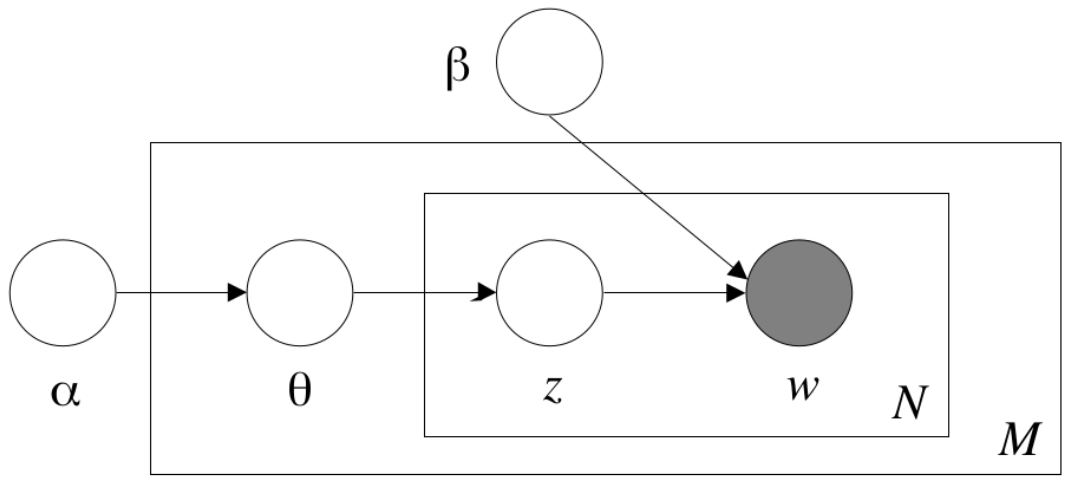
\includegraphics[width=\linewidth]{chapter12/lda.png}
  \caption{Latent Dirichlet Allocation in `Plate Model' notation \citep[fig. 1]{blei03}}\label{fig:lda}
\end{figure}

\reffig{lda} is a more formal notation of the same generative model.
Starting from the left, for each document you pick a set of topics $\Theta$.
This set of topics is drawn from a \concept{Dirichlet distribution} which itself has a parameter $\alpha$
(see note).
Next, for each word you select a single topic $z$ from the topics in that document.
Finally, you pick an actual word $w$ from the words in that topic, again controlled by a paramter $\beta$ (see note).

Now, if we would know which words and documents are in which topics, we could start generating the documents in the corpus.
In reality, of course, we have the reverse situation:
we know the documents, and we want to know the topics.
Thus, the task of LDA is to find the parameters that have the highest chance of generating these documents.
Since only the word frequencies are observed, this is a latent variable model where we want to find the
most likely values for the (latent) topic $z$ for each word in each document. 

Unfortunately, there is no simple analytic solution to calculate these topic assignments
like there is for OLS regression.
Thus, like other more complicated statistical models such as multilevel regression,
we need to use an iterative estimation that progressively optimizes the assignment to improve the fit until it converges.

An estimation method that is often used for LDA is Gibbs sampling.
Simply put, this starts with a random assignment of topics to words.
Then, each iteration, it reconsiders each words and recomputes what likely topics for that word are
given the other topics in that document and the topics that word occurs in in other documents.
Thus, if a document already contains a number of words about placed in a certain topic,
a new word is more likely to be placed in that topic as well.
After enough iterations, this converges to a solution. 

\note{\textbf{The Dirichlet Distribution and its Hyperparameters}
  The Dirichlet distribution can be seen as a distribution over multinomial distributions,
  that is, every draw from a dirichlet distribution results in a multinomial distribution.
  An easy way to visualize this is to see the dirichlet distribution as a bag of dice.
  You draw a die from the bag, and each die is a distribution over the numbers one to six.

  This distribution is controlled by a parameter called alpha ($\alpha$),
  which is often called a \concept{hyperparameter} because it is a parameter that controls how other parameters
  (the actual topic distributions) are estimated, similar to e.g. the learning speed in many machine learning models.
  This alpha hyperparameter controls what kind of dice there are in the bag.
  A high alpha means that die are generally fair, i.e., give a uniform multinomial distribution.
  For topic models, this means that documents will in general contain an even spread of multiple topics.
  A low apha means that each die is unfair in the sense of having a strong preference for some number(s), as if these numbers are weighed down. You can then draw a die that prefers ones, or a die that prefers sixes.
  For topic models this means that each document tends to have one or two dominant topics.
  Finally, alpha can be symmetric (meaning dice are unfair, but randomly, so in the end each topic has the same chance)
  or assymetric (this are still unfair, and now also favour some topics more than others).
  This would correspond to some topics being more likely to occur in all documents.
  
  In our experience, most documents actually do have one or two dominant topics,
  and some topics are actually more prevalent across many documents then others
  -- especially if you consider that procedural words and boilerplate also need to be fit into a topic unless they are filtered out beforehand.
  Thus, we would generally recommend a relatively low and asymmetric alpha,
  and in fact Gensim by default uses an algorithm to find an alpha that corresponds to this recommendation.
  In R, we would recommend picking a lower alpha than the default value, probably around $\alpha=5/K$,
  and optionally try using an asymmetric alpha if you find some words that occur across multiple topics. 

  To get a more intuitive understanding of the effects of alpha,
  please see \url{http://cssbook.net/lda} for additional material and visualizations.
  }

\subsection{Fitting an LDA model}


\begin{ccsexample}
\doublecodex{chapter12/lda1}
\codex[caption=Output (from R)]{chapter12/lda1.r.out}
\doublecodex{chapter12/lda2}
\codexoutputtable{chapter12/lda2.r}
\caption{LDA Topic Model of Obama's State of the Union speeches}\label{ex:lda}
\end{ccsexample}

\refex{lda} shows how you can fit an LDA model in Python or R.
As example data, we use Obama's State of the Union Speeches using the corpus introduced in \refchap{dtm}.
Since such a speech generally touches on many different topics, we choose to first split by paragraph
as these will be more semantically coherent (for Obama, at least).
In R, we se the \fn{corpus\_reshape} function to split the paragraphs,
while in Python we use \pandas' \fn{str.split}, which creates a list or paragraphs for each text,
which we then convert into a paragraph per row using \fn{explode}.
Converting this to a DTM we get a reasonably sized matrix of 738 paragraphs and 746 unique words.

Next, we fit the actual LDA model using the package \pkg{gensim} (Python) and \pkg{topicmodels}.
Before we can do this, we need to convert the DTM format into a format accepted by that package.
For Python, this is done using the \fn{Sparse2Corpus} helper function while in R this is done with the \quanteda\ \fn{convert} function.
Then, we fit the model, asking for 10 topics to be identified in these paragraphs.
There are three things to note in this line.
First, we specify a \concept{random seed} of 123 to make sure the analysis is replicable.
Second, we specify an `assymetric' of \verb|1/1:10|, meaning the first topic has alpha 1, the second 0.5, etc.
-- see the note on hyperparameters for more information. 
Third, for Python we also need to specify the vocabulary names since these are not included in the DTM.

The final line generates a data frame of top words per topic for first inspection
(which in Python requires separating the words from their weights in a list comprehension and converting it to a dataframe for easy viewing).
As you can see, most topics are interpretable and somehwat coherent: For example, topic 1 seems to be about education and jobs,
while topic two is health care. You also see that the word `job' occurs in multiple topics (presumably because unemployment was a pervasive concern during Obama's tenure).
Also, some topics like topic 3 are more difficult to interpret from this table.
A possible reason for this is that not every paragraph actually has policy content.
For example, the first paragraph of his first State of the Union was:
\emph{`Madam Speaker, Mr. Vice President, Members of Congress, the First Lady of the United States -- she's around here somewhere'}.
None of these words really fit a `topic' in the normal meaning of that term,
but all of these words need to be assigned a topic in LDA.
Thus, you often see `procedural' or `boilerplate' topics such as topic 3 occurring in LDA outputs. 

Finally, note that we showed the R results here. As \pkg{gensim} uses a different estimation algorithm
(and \sklearn\ uses a different tokenizer and stopword list), results will not be identical,
but should be mostly similar. 

\subsection{Analysing topic model results}

\begin{ccsexample}
\doublecodex{chapter12/ldaresults1}
\codexoutputtable{chapter12/ldaresults1.r}
\doublecodex{chapter12/ldaresults2}
\codex[caption=Output (from R)]{chapter12/ldaresults2.r.out}
\caption{Analysing and inspecting LDA results}\label{ex:ldaresults}
\end{ccsexample}


\refex{ldaresults} shows how you can combine the LDA results (topics per document)
with the original document metadata.
This could be your starting point for substantive analysis of the results,
for example to investige relations between topics or between e.g. time or partisanship and topic use.

You can also use this to find specific documents for reading.
For example, we noted above that topic 3 is difficult to interpret.
As you can see in the table in \refex{ldaresults} (which is sorted by value of topic 3),
most of the high scoring documents are the first paragraph in each speech,
which do indeed contain the ``Madam speaker'' boilerplate noted above.
The other three documents are all calls for bipartisanship and support.
As you can see from this example, carefully inspecting the top documents for each topic
is very helpful for making sense of the results.


\subsection{Validating and inspecting topic models}

As we saw in the previous subsection, running a topic model is relatively easy.
However, that doesn't mean that the resulting topic model will always be useful.
As with all text analysis techniques, \concept{validation} is the key to good analysis:
are you measuring what you want to measure? And how do you know?

For topic modeling (and arguably for all text analysis),
the first step after fitting a model is inspecting the results and establishing face validity.
Top words per topic such as listed above are a good place to start with this,
but we would really encourage you to also look at the top documents per topic to better understand how words are used in context.
Also, it is good to inspect the relations between topics and look at documents that load high on multiple topics to understand the relation.

If the only goal is to get a explorative understanding of the corpus,
for example as a first step before doing a dictionary analysis or manual coding,
just face validity is probably sufficient.
For a more formal validation, however, it depends on the reason for using topic modeling.

If using topic modeling in a true unsupervised sense, i.e. without a predefined analytic schema in mind,
it is difficult to assess whether the model measures what you want to measure --
because the whole point is that you don't know what you want to measure.
That said, however, you can have the general criteria that the model needs to be \emph{coherence}
and \emph{interpretability}, meaning that words and documents that share a topic
are also similar semantically. 

In their excellent paper on the topic, \citet{chang09} propose two formal tasks to judge this
using manual (or crowd) coding: in \emph{word intrusion}, a coder is asked to pick the `odd one out' from a list
where one other word is mixed in a group of topic words.
In \emph{topic intrusion}, the coder is presented with a document and a set of topics that occur in the document,
and is asked to spot the one topic that was not present according to the model.
In both tasks, if the coder is unable to identify the intruding word or topic, apparently the model does not fit
our intuitive notion of `aboutness' or semantic similarity.
Perhaps their most interesting finding is that goodness-of-fit measures like perplexity
are actually not good predictors of the interpretability of the resulting models.

If you are using topic models in a more confirmatory manner,
that is, if you wish the topics to match some sort of predefined categorization,
you should use regular gold standard techniques for validation:
code a sufficiently large random sample of documents with your predefined categories,
and test whether the LDA topics match those categories.
In general, however, in such cases it is a better idea to use a dictionary or supervised analysis technique
as topic models often do not exactly capture our categories.


\subsection{Beyond LDA}

This chapter focused on regular or `vanilla' LDA topic modeling.
Since the seminal publication, however, a large amount of variations and extensions on LDA have been proposed.
These include dynamic topic models (which incorporate time; \cite*{dynamiclda}),
correlated topic models (which explicitly model correlation between topics; \cite{correlatedlda}).
Although it is beyond the scope of this book to describe these models in detail,
the interested reader is encouraged to learn more about these models.

Especially noteworthy are \concept{Structural Topic Models} (R package \pkg{stm}; \cite*{stm}),
which allows you to model covariates as topic or word predictors.
This allows you, for example, to model topic shifts over time or
different words for the same topic based for e.g. Republican or Democrat presidents. 

Python users should check out Hierarchical Topic Modeling \citep{hierarchicallda}.
In hierarchical topic modeling, rather than the researcher specifying a fixed number of topics,
the model returns a hierachy of topics from few general topics to a large number of specific topics,
allowing for a more flexible exploration and analysis of the data. 


